\chapter{刚体力学}\label{ch:b2:rigid-body-mechanics}

从路边观察自行车的车轮：靠近路面的辐条几乎
静止、轮廓清晰；位于顶部的辐条则模糊一片，其运动速度是骑车人速度的两倍。
车轮上每一点的速度各不相同，
但车轮是一个整体——各点间距离保持不变，这一约束
把所有运动归结为两个矢量：一个平动，
一个转动。本科一年级分册讨论了固体绕定轴转动这一特殊情形，
本章给出刚体的一般运动学、
动能与角动量、刚体的运动定律，
以及支配每一个车轮、轮胎、刹车和梯子的规律，
即库仑干摩擦定律。

\section{刚体运动学}

\begin{definition}[刚体]\label{def:b2:rigid-body-mechanics:solid}
\index{刚体}
称\emph{刚体}（或固体）为一个质点系，其中两点间的
距离保持不变：$\|\vect{AB}\|$ 与时间无关，
对其中任意两点 $A$、$B$。若刚体上每一点都静止于某参考系中，
则称该参考系为\emph{固连于刚体的参考系}。
\end{definition}

\begin{theorem}[刚体的速度场]\label{thm:b2:rigid-body-mechanics:field}
\index{转动矢量}\index{速度场（刚体）}
在每一时刻，存在矢量 $\vect\Omega$，称为刚体的\emph{转动
矢量}（单位为 \unit{rad/s}），使得刚体上任意两点
$A$ 与 $M$ 的速度在参考系 $\mathcal R$ 中满足
\[
\vect v_M = \vect v_A + \vect\Omega\wedge\vect{AM} .
\]
$\vect\Omega$ 与 $A$ 的选取无关；固连于刚体的矢量 $\vect u$
满足 $\dd\vect u/\dd t = \vect\Omega\wedge\vect u$。
\end{theorem}

\begin{proof}
设 $(\vect e_1, \vect e_2, \vect e_3)$ 为固连于刚体的
一组标准正交基。由 $\vect e_i\cdot\vect e_j = \delta_{ij}$，
系数 $a_{ij} = \dot{\vect e}_i\cdot\vect e_j$ 满足 $a_{ij} + a_{ji} = 0$：
映射 $\vect u \mapsto \dot{\vect u}$ 的矩阵（对固连于刚体的 $\vect u$，
即 $\vect u = \sum u_i\vect e_i$，其中 $u_i$ 为常数）是
反对称的；而一个反对称的 $3\times3$ 矩阵恰为
映射 $\vect u \mapsto \vect\Omega\wedge\vect u$ 的矩阵，其中 $\Omega_1 = a_{23}$，
$\Omega_2 = a_{31}$，$\Omega_3 = a_{12}$。将其作用于 $\vect u =
\vect{AM}$，得 $\vect v_M - \vect v_A = \vect\Omega\wedge\vect{AM}$。
若 $\vect\Omega'$ 亦满足同样的关系，则 $(\vect\Omega - \vect\Omega')\wedge
\vect{AM} = \vect 0$ 对每个 $M$ 成立，故 $\vect\Omega' = \vect\Omega$。
\end{proof}

\begin{remark}[三种运动]\label{rem:b2:rigid-body-mechanics:motions}
\index{平动}\index{定轴转动}
\emph{平动}：$\vect\Omega = \vect 0$，所有点具有相同的
速度（不一定是直线运动：摩天轮的座舱
沿圆周平动）。\emph{定轴转动}，轴 $\Delta$：
$\Delta$ 上的点静止，$\vect\Omega = \omega\,\vect e_\Delta$，
距轴为 $r$ 的点沿圆周运动，速率为
$r|\omega|$——即本科一年级分册所讨论的情形。
一般运动是两者的结合：$\vect v_M = \vect v_G + \vect\Omega\wedge\vect{GM}$，
即以质心的速度平动，并绕
$G$ 转动。
\end{remark}

\begin{definition}[无滑动滚动]\label{def:b2:rigid-body-mechanics:rolling}
\index{无滑动滚动}\index{滑动速度}
两个固体 $S_1$ 与 $S_2$ 在一点 $I$ 处接触。$S_1$ 相对于 $S_2$ 的\emph{滑动
速度}为 $\vect v_{\text{滑动}} = \vect v_{I \in S_1}
- \vect v_{I \in S_2}$，即此时于
$I$ 处重合的两个物质点的速度之差。$S_1$ 在 $S_2$ 上\emph{无
滑动滚动}，当 $\vect v_{\text{滑动}} = \vect 0$ 时。对于
半径为 $R$ 的车轮沿固定地面无滑动滚动，
轮心速度为 $v_G$，角速度为 $\omega$，则条件为
$v_G = R\omega$（符号的选取使得向右滚动的车轮沿
顺时针转动）。
\end{definition}

\begin{proof}
由\cref{thm:b2:rigid-body-mechanics:field}，对车轮上的 $G$
与接触点 $I$：$\vect v_{I\in S_1} = \vect v_G + \vect\Omega
\wedge\vect{GI}$；取 $\vect v_G = v_G\vect e_x$，$\vect\Omega = -\omega
\vect e_z$，$\vect{GI} = -R\vect e_y$，则上式为 $(v_G - R\omega)\vect e_x$，
它必须为零。
\end{proof}

\begin{example}[滚动车轮的速度场]\label{ex:b2:rigid-body-mechanics:wheel}
对于滚动的车轮，$\vect v_M = \vect\Omega\wedge\vect{IM}$：在每一
时刻，车轮\emph{绕其接触点转动}。接触
点静止，轮心以 $v = R\omega$ 运动，顶部以 $2v$ 运动，而
轮缘上高度为 $h$ 的一点以 $\omega\sqrt{2Rh}$ 运动，
且速度垂直于 $\vect{IM}$。气门嘴的轨迹为摆线；
从胎面甩出的石子，以轮缘该点的速率飞出，最大可达 $2v$
——这正是卡车挡泥板如此重要的原因。
\end{example}

\begin{omfigure}
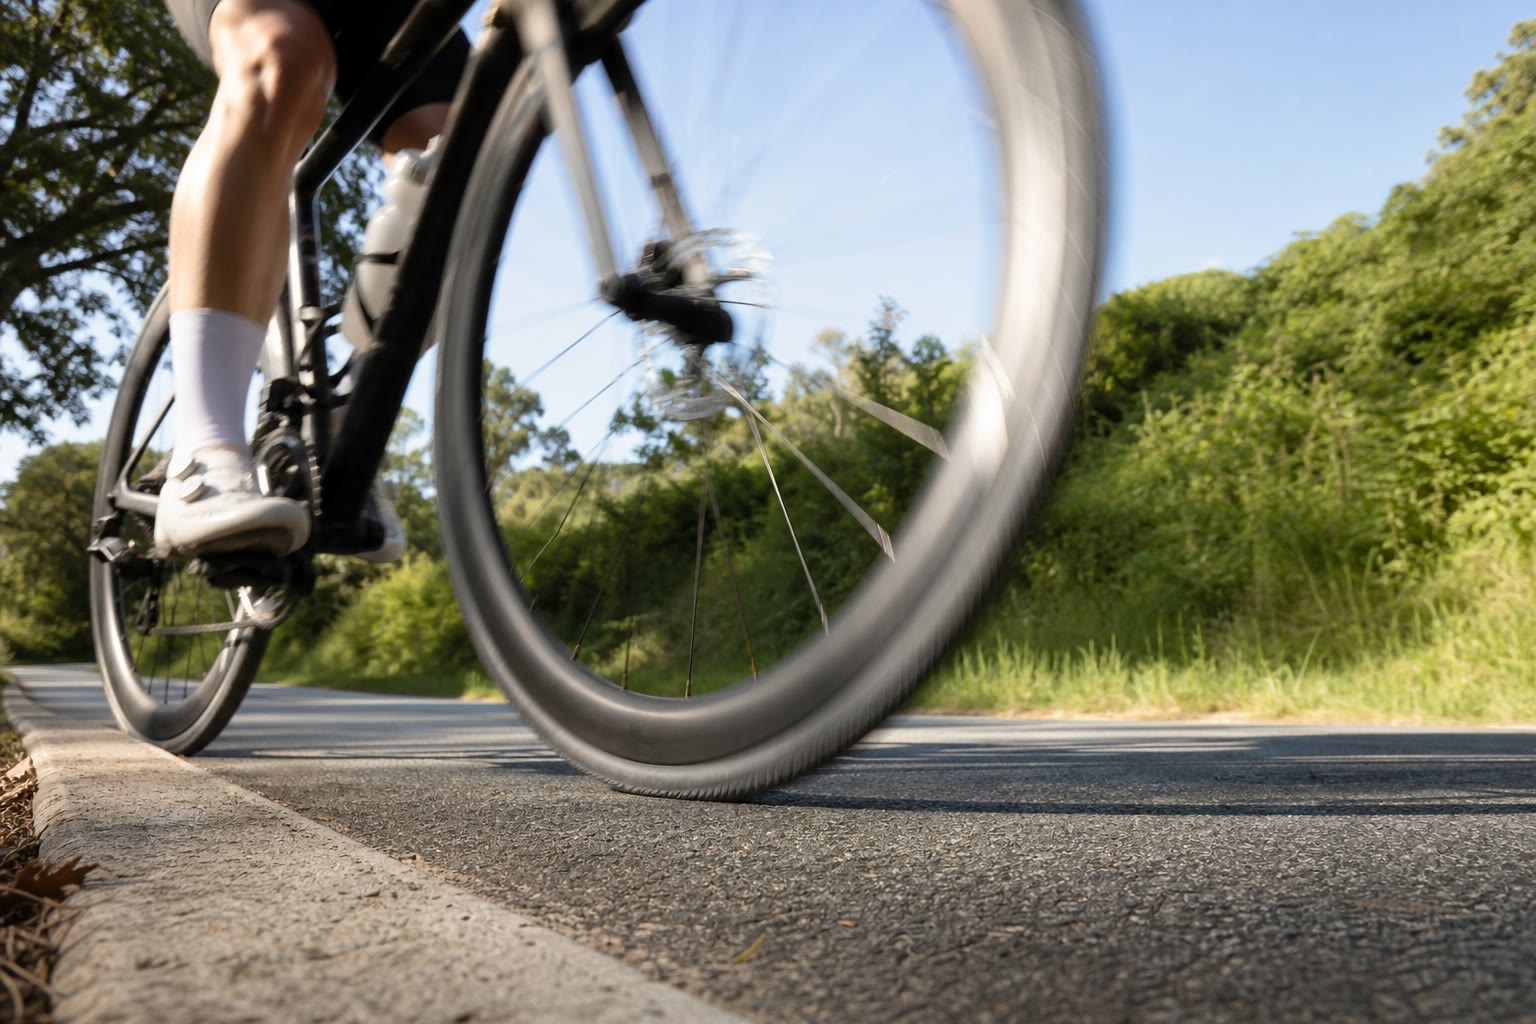
\includegraphics[width=0.58\linewidth]{images/book4/ai/b4-01-bicycle-wheel-blur.jpg}

{\small 慢速快门拍下的车轮：靠近路面、几乎静止的辐条保持清晰；位于顶部、以自行车两倍速度运动的辐条则模糊。}
\end{omfigure}


\begin{omfigure}
\begin{tikzpicture}[font=\small, x=1cm, y=1cm, >=Stealth]
  \begin{scope}
    \draw[thick] (-2.6,0) -- (2.6,0);
    \draw[omDef, thick] (0,1.5) circle (1.5);
    \fill (0,1.5) circle (1.5pt) node[below left, font=\footnotesize] {$G$};
    \fill (0,0) circle (1.5pt) node[below, font=\footnotesize] {$I$};
    \draw[omThm, very thick, ->] (0,1.5) -- (1.2,1.5) node[above, font=\footnotesize] {$\vect v_G$};
    \draw[omThm, very thick, ->] (0,3.0) -- (2.4,3.0) node[pos=0.35, above, font=\footnotesize] {$2\vect v_G$};
    \draw[omThm, very thick, ->] (1.5,1.5) -- (2.7,0.3) node[right, font=\footnotesize] {$\sqrt2\,v_G$};
    \draw[omThm, very thick, ->] (-1.5,1.5) -- (-0.3,2.7) node[above left, font=\footnotesize] {$\sqrt2\,v_G$};
    \draw[omThm, thick, ->] (1.06,0.44) -- (1.41,-0.41);
    \draw[omThm, thick, ->] (-1.06,0.44) -- (-0.71,1.29);
    \node[omThm, font=\footnotesize] at (0.3,0.35) {$\vect v_I = \vect 0$};
    \draw[omProp, ->] (-0.5,2.1) arc[start angle=130, end angle=50, radius=0.75] node[midway, above, font=\footnotesize] {$\omega$};
  \end{scope}
  \begin{scope}[xshift=7.6cm]
    \draw[thick] (-2.6,0) -- (2.6,0);
    \draw[omDef, thick] (0,1.5) circle (1.5);
    \fill (0,0) circle (1.5pt) node[below, font=\footnotesize] {$I$};
    \fill (0,1.5) circle (1.5pt);
    \draw[omThm, ->] (0,1.5) -- ($(0,1.5)!0.45!90:(0,0)$);
    \foreach \a in {30,60,...,330} {
      \coordinate (M) at ({1.5*cos(\a)},{1.5+1.5*sin(\a)});
      \draw[omThm, ->] (M) -- ($(M)!0.45!90:(0,0)$);
    }
    \draw[dashed, omExo] (0,0) -- (1.3,2.25);
    \fill (1.3,2.25) circle (1.2pt) node[right, font=\footnotesize] {$M$};
    \node[font=\footnotesize] at (0,-0.8) {$\vect v_M = \vect\Omega\wedge\vect{IM}$};
    \node[font=\footnotesize, align=center] at (0,3.6) {瞬时绕接触点 \\转动};
  \end{scope}
\end{tikzpicture}

{\small 一个无滑动滚动的车轮。左图：若干点的
速度——接触点 $I$ 处为零，中心处 $v_G = R\omega$，
顶部为 $2v_G$。右图：每个速度都垂直于连接该点与接触点的线段，
并与该点到 $I$ 的线段长度成正比：每一瞬时，
车轮都绕接触点转动。}
\end{omfigure}

\section{刚体的动力学量}

\begin{proposition}[动量、角动量、动能]\label{prop:b2:rigid-body-mechanics:kinetic}
\index{转动惯量}\index{角动量（刚体）}\index{动能（刚体）}
设刚体质量为 $M$，质心为 $G$，在参考系 $\mathcal R$ 中：
\begin{itemize}
  \item 其动量为 $\vect p = M\vect v_G$；
  \item 若刚体绕轴 $\Delta$ 转动（该轴在 $\mathcal R$ 中固定，或
        过 $G$ 且方向固定），角速度为
        $\omega$，则其\emph{沿}该轴的角动量为
        $L_\Delta = J_\Delta\,\omega$，其中
        \[
        J_\Delta = \sum_i m_i r_i^2 = \int r^2\,\dd m
        \]
        即其\emph{转动惯量}（对轴 $\Delta$ 而言；$r$ 为到轴的
        距离；单位 \unit{kg.m^2}）；
  \item 其动能为（柯尼希）$E_k = \tfrac12Mv_G^2 +
        E_k^*$，其中质心参考系中的动能为
        $E_k^* = \tfrac12J_{G}\omega^2$，即以 $\omega$ 绕
        过 $G$ 的轴转动时——而 $E_k = \tfrac12J_\Delta\omega^2$ 适用于
        绕定轴 $\Delta$ 的转动。
\end{itemize}
\end{proposition}

\begin{proof}
动量定理与柯尼希定理已在本科一年级分册中证明，
对任意质点系成立。对绕 $\Delta$ 的转动（轴过 $O$），
距轴为 $r_i$ 的质点，在绕轴的圆周上速率为 $r_i\omega$；
其对 $O$ 的角动量在 $\vect e_\Delta$ 上的投影为
$m_ir_i^2\omega$（其余分量对对称
刚体相互抵消，此处不需要）；求和。动能：$\sum\tfrac12m_ir_i^2
\omega^2$。
\end{proof}

\begin{remark}[在本阶段不加证明地承认]\label{rem:b2:rigid-body-mechanics:tensor}
对任意转动 $\vect\Omega$，一般情况下完整的矢量 $\vect L_G$
并不与 $\vect\Omega$ 平行：$\vect L_G = \mathbf J\,\vect\Omega$，
其中 $\mathbf J$ 为\emph{惯量张量}，是一个对称矩阵，其
特征向量即主轴。本章中的每个刚体
都绕定轴或过 $G$ 的对称轴转动，对于这类情形，
$\vect L = J\vect\Omega$ 精确成立；一般情形属于本科三年级
分册的内容。
\end{remark}

\begin{proposition}[转动惯量]\label{prop:b2:rigid-body-mechanics:inertia}
\index{惠更斯定理}\index{平行轴定理}
对质量为 $M$ 的均匀刚体，绕过 $G$ 的轴：细杆
长为 $\ell$（轴与杆垂直），$J = \tfrac1{12}M\ell^2$；细圆环
或圆柱薄壳，半径为 $R$（沿自身轴），$J = MR^2$；圆盘或
实心圆柱，$J = \tfrac12MR^2$；实心球，$J = \tfrac25MR^2$；
球壳，$J = \tfrac23MR^2$。\emph{惠更斯定理}（平行轴）：对
任一轴 $\Delta$ 平行于轴 $\Delta_G$，后者过 $G$，
两轴间距为 $d$，则
\[
J_\Delta = J_{\Delta_G} + Md^2 .
\]
\end{proposition}

\begin{proof}
细杆：$\int_{-\ell/2}^{\ell/2}x^2\,(M/\ell)\dd x = M\ell^2/12$。圆盘：取质量为
$(2M/R^2)r\,\dd r$ 的圆环，$\int_0^R r^2(2M/R^2)r\,\dd r = MR^2/2$。球：由
对称性，$J = \tfrac23\int r^2\dd m$（$r$ 为到球心的距离，
因为在三个轴上取平均，$x^2 + y^2 = \tfrac23(x^2 + y^2 + z^2)$
），且 $\int r^2\dd m = \int_0^R r^2(3M/R^3)r^2\dd r = \tfrac35MR^2$。
惠更斯定理：取 $\vect r_i$ 为由 $\Delta$ 指向 $m_i$、垂直于
轴的矢量，并记 $\vect r_i = \vect d + \vect r_i^*$，则 $\sum m_ir_i^2 = Md^2
+ 2\vect d\cdot\sum m_i\vect r_i^* + \sum m_ir_i^{*2}$，其中中间的和式
由 $G$ 的定义为零。
\end{proof}

\begin{example}[飞轮]\label{ex:b2:rigid-body-mechanics:flywheel}
一个钢制圆盘，质量为 \qty{50}{kg}，半径为 \qty{30}{cm}：$J = \tfrac12 \times
50 \times 0.09 = \qty{2.25}{kg.m^2}$；转速为 \qty{3000}{rpm}（$\omega =
\qty{314}{rad/s}$）时，其储存能量 $\tfrac12J\omega^2 = \qty{111}{kJ}$，相当于
一辆以 \qty{50}{km/h} 行驶的小汽车的动能。储能飞轮
在真空中以 \qty{50000}{rpm} 旋转碳纤维转子，置于
磁悬浮轴承上：能量随 $\omega^2$ 增长，其极限取决于
轮缘的抗拉强度。
\end{example}

\section{刚体的动力学}

\begin{theorem}[刚体的运动定律]\label{thm:b2:rigid-body-mechanics:laws}
\index{角动量定理（刚体）}\index{作用于刚体的力的功率}
在伽利略参考系中，对受外力 $\vect F_i$
（作用于点 $A_i$）的刚体：
\begin{enumerate}
  \item （动量）$M\,\dd\vect v_G/\dd t = \sum\vect F_i$；
  \item （对 $G$ 或定点 $O$ 的角动量）
        $\dd\vect L_G/\dd t = \sum\vect{GA_i}\wedge\vect F_i$；投影到
        定轴 $\Delta$ 上，或在过 $G$ 且方向固定的轴上（刚体沿
        该方向以 $\omega$ 转动）：
        $J_\Delta\,\dd\omega/\dd t = \mathcal M_\Delta$，即外力
        对该轴的力矩之和；
  \item （功率）作用于刚体的一组力的功率为
        $\mathcal P = \vect R\cdot\vect v_A + \vect{\mathcal M}_A\cdot
        \vect\Omega$ 对刚体上任一点 $A$ 成立，其中 $\vect R$ 为
        诸力之和，$\vect{\mathcal M}_A$ 为其
        对 $A$ 的总力矩；\emph{刚体内力的
        功率为零}，且 $\dd E_k/\dd t = \mathcal P_{\text{外}}$。
\end{enumerate}
\end{theorem}

\begin{proof}
(1) 和 (2) 即本科一年级分册中关于质点组的定理
（关于 $G$ 的角动量定理在 $G$ 加速时仍然成立，
因为质心参考系的惯性力对 $G$ 的力矩为零）。
(3) 记 $\vect v_{A_i} = \vect v_A + \vect\Omega
\wedge\vect{AA_i}$: $\sum\vect F_i\cdot\vect v_{A_i} = \vect R\cdot\vect v_A
+ \sum\vect F_i\cdot(\vect\Omega\wedge\vect{AA_i}) = \vect R\cdot\vect v_A +
\vect\Omega\cdot\sum\vect{AA_i}\wedge\vect F_i$（混合积）。内力
之和及其总力矩均为零（作用与反作用，同一直线），
故刚体上内力的功率为零——\emph{并非}可变形
系统的情形。于是动能定理只保留外力功率。
\end{proof}

\begin{definition}[理想转轴]\label{def:b2:rigid-body-mechanics:pivot}
\index{理想转轴}\index{轴承}
刚体绕固定轴 $\Delta$ 在\emph{理想转轴}中转动
（即理想轴承），当轴承的接触力
对 $\Delta$ 的力矩为零时，其功率为零（$\vect v_A = \vect 0$
在轴上，$\mathcal M_\Delta = 0$）。实际轴承会附加一个摩擦
力矩 $-\Gamma_f\operatorname{sgn}\omega$，或黏性力矩 $-h\omega$。
\end{definition}

\begin{proposition}[物理摆]\label{prop:b2:rigid-body-mechanics:pendulum}
\index{物理摆}\index{复摆}
质量为 $M$ 的刚体绕水平固定轴 $\Delta$ 在
理想转轴中摆动，其质心到轴的距离为 $d$。记
$\theta$ 为 $\vect{OG}$ 与竖直向下方向的夹角，
\[
J_\Delta\ddot\theta = -Mgd\sin\theta ,
\]
于是小振动的周期为 $T = 2\pi\sqrt{J_\Delta/Mgd}$
——与长度为 $\ell_{\text{平衡}} = J_\Delta/Md$ 的单摆周期相同。
\end{proposition}

\begin{proof}
关于 $\Delta$ 的角动量定理：重力的力矩为
$-Mgd\sin\theta$，支点的力矩为零。线性化。
\end{proof}

\begin{example}[米尺]\label{ex:b2:rigid-body-mechanics:rule}
一根一端为支点的米尺：$J = \tfrac13M\ell^2$（惠更斯由
$\tfrac1{12}M\ell^2$ 出发），$d = \ell/2$，$\ell_{\text{等效}} = \tfrac23\ell =
\qty{0.667}{m}$，且 $T = \qty{1.64}{s}$——整根米尺构成的摆
比悬挂于其中心的质点慢（\qty{1.42}{s}），并比悬挂于其一端的质点快（\qty{2.0}{s}）。
比挂在其一端的质点快（\qty{2.0}{s}）。
\end{example}

\begin{omfigure}
\begin{tikzpicture}[font=\small, x=1cm, y=1cm, >=Stealth]
  \begin{scope}
    \fill[pattern=north east lines] (-0.6,3.2) rectangle (0.6,3.45); \draw[thick] (-0.6,3.2) -- (0.6,3.2);
    \fill (0,3.1) circle (2pt) node[left, font=\footnotesize] {$O$};
    \draw[dashed] (0,3.1) -- (0,0.2);
    \draw[omDef, very thick, rotate around={25:(0,3.1)}] (-0.12,3.1) rectangle (0.12,0.3);
    \draw[dashed, omExo] (0,3.1) -- ($(0,3.1)+({2.0*sin(25)},{-2.0*cos(25)})$);
    \coordinate (G) at ({0+1.4*sin(25)},{3.1-1.4*cos(25)});
    \fill[omThm] (G) circle (2pt) node[right, font=\footnotesize] {$G$};
    \draw[omThm, very thick, ->] (G) -- ($(G)+(0,-1.0)$) node[below, font=\footnotesize] {$M\vect g$};
    \draw[<->, omExo] (0,1.5) arc[start angle=-90, end angle=-65, radius=1.6] node[midway, below, font=\footnotesize] {$\theta$};
    \node[font=\footnotesize] at (2.1,2.3) {$J_\Delta\ddot\theta = -Mgd\sin\theta$};
    \draw[<->, omExo] (-0.5,3.1) -- ($(-0.5,3.1)+(0,-1.28)$) node[midway, left, font=\footnotesize] {$d$};
  \end{scope}
  \begin{scope}[xshift=7cm]
    \draw[thick] (-2.5,0) -- (2.5,0);
    \draw[omDef, thick] (0,1.2) circle (1.2);
    \fill (0,1.2) circle (1.5pt);
    \draw[omThm, very thick, ->] (0,1.2) -- (0,-0.3) node[right, font=\footnotesize] {$M\vect g$};
    \draw[omProp, very thick, ->] (0,0) -- (0,1.0) node[left, font=\footnotesize, pos=0.7] {$\vect N$};
    \draw[omExo, very thick, ->] (0,0) -- (-1.0,0) node[below, font=\footnotesize] {$\vect T$};
    \draw[very thick, ->] (0.3,2.6) -- (1.5,2.6) node[right, font=\footnotesize] {$\vect F$};
    \draw[omDef, ->] (-0.5,1.7) arc[start angle=130, end angle=50, radius=0.75] node[midway, above, font=\footnotesize] {$\omega$};
    \node[font=\footnotesize, align=left] at (0,-0.9) {无滑动滚动：$|T| \le fN$};
  \end{scope}
\end{tikzpicture}

{\small 左：物理摆——重力关于支点的力矩驱动转动，
支点处的力没有力矩。右图：
水平地面上滚动车轮所受的力：重力、法向
反作用力 $\vect N$ 和接触点处的切向摩擦力 $\vect T$，
其大小受库仑定律限制。}
\end{omfigure}

\section{接触力与库仑摩擦}

\begin{definition}[接触力、法向与切向分量]\label{def:b2:rigid-body-mechanics:contact}
\index{法向力}\index{摩擦力}
支座在接触点 $I$ 处对刚体施加的力分解为
一个\emph{法向力} $\vect N$，垂直于公切面，
并指向刚体（$N \ge 0$：支座只能推
，不能拉），以及位于切平面内的\emph{切向分量} $\vect T$，
即\emph{摩擦力}。
\end{definition}

\begin{theorem}[库仑摩擦定律]\label{thm:b2:rigid-body-mechanics:coulomb}
\index{库仑摩擦定律}\index{摩擦因数}\index{静摩擦力}\index{动摩擦力}
对于接触的两个干固体，其\emph{摩擦因数} $f$
由材料及表面状态决定，而不取决于
接触面积，（在很好的近似下）也不取决于速率：
\begin{itemize}
  \item 若两固体相互滑动（$\vect v_{\text{滑动}} \ne
        \vect 0$），则摩擦力与滑动速度方向相反，
        大小为 $\|\vect T\| = f\|\vect N\|$（动摩擦力）；
  \item 若不滑动，$\|\vect T\| \le f\|\vect N\|$（静
        摩擦力）：此时摩擦力为其他运动定律所要求的
        值，且须在该界限内，其方向
        事先未知。
\end{itemize}
\emph{理想接触}即理想化情形 $f = 0$：$\vect T = \vect 0$。
\end{theorem}
\admitted

\begin{remark}[阅读库仑定律]\label{rem:b2:rigid-body-mechanics:reading}
\index{摩擦锥}
第一定律是等式，第二定律是不等式——这正是
摩擦问题的全部难点。\emph{方法}是
\emph{假设}不滑动，解出 $\vect T$ 和 $\vect N$，并
\emph{检验} $\|\vect T\| \le f\|\vect N\|$；若检验不通过，则
固体滑动，$\|\vect T\| = f\|\vect N\|$，方向与滑动方向相反，然后
重新求解。从几何上看，接触力必须位于
\emph{摩擦锥}之内，其半顶角为 $\varphi$，且 $\tan\varphi
= f$。典型数值：干燥沥青上橡胶的 $f \approx 0.8$--$1$，湿沥青上
为 $0.4$--$0.6$，冰面上为 $0.1$；钢对钢，干燥时为 $0.15$，
涂油时为 $0.05$。实际中静摩擦因数略大于
动摩擦因数，这正是打滑一旦开始便难以制动的原因。
\end{remark}

\begin{proposition}[接触力的功率；无滑动滚动]\label{prop:b2:rigid-body-mechanics:power}
\index{滚动摩擦}
固定支承上运动的固体所受接触力的功率为
$\mathcal P = \vect T\cdot\vect v_{I\in S}$（法向力与
接触点的速度垂直，而该速度位于
切平面内）。在\emph{无滑动滚动}中，此功率为零：
摩擦力不做功，但它对运动可能至关重要。
滑动时功率为 $-f N v_{\text{滑动}} < 0$：产生热量。
\end{proposition}

\begin{proof}
$\mathcal P = (\vect N + \vect T)\cdot\vect v_{I\in S}$，且 $\vect
v_{I\in S} = \vect v_{\text{滑动}}$ 位于切平面内，故只有
$\vect T$ 有贡献：滑动速度为零时它为零，而
固体滑动时为 $-fNv_{\text{滑动}}$（$\vect T$ 与 $\vect
v_{\text{滑动}}$ 方向相反）。实际滚动会因轮胎与地面
的形变而有少量耗散（\emph{滚动摩擦}，可用小力矩
$\Gamma_r = \mu_rNR$ 或等效力 $\mu_rN$ 描述，其中
对于道路上的轮胎，$\mu_r \approx 0.01$）：这是另一种小得多的
效应。
\end{proof}

\begin{method}[沿斜面滚下的固体]\label{met:b2:rigid-body-mechanics:incline}
\index{沿斜面滚动}
一个均匀固体，半径为 $R$、质量为 $M$、绕其轴的转动惯量为 $J =
kMR^2$（$k = 1$ 为薄圆环，$\tfrac12$ 为圆盘，$\tfrac25$ 为球体），
从倾角为 $\alpha$、摩擦因数为
$f$ 的斜面上释放。假设无滑动滚动：
\begin{enumerate}
  \item 沿斜面方向的动量：$M\dot v = Mg\sin\alpha - T$；法向：
        $N = Mg\cos\alpha$；
  \item 对 $G$ 的角动量：$kMR^2\dot\omega = TR$；
  \item 无滑动：$v = R\omega$，故 $T = kM\dot v$，且
        \[
        \dot v = \frac{g\sin\alpha}{1 + k} , \qquad T = \frac{k}{1 + k}\,
        Mg\sin\alpha ;
        \]
  \item 检验：$T \le fN \iff \tan\alpha \le f\,\dfrac{1 + k}{k}$。
        超过此斜率后固体滑动，$T = fMg\cos\alpha$，$\dot v =
        g(\sin\alpha - f\cos\alpha)$，$\dot\omega = fg\cos\alpha/kR$。
\end{enumerate}
能量检验（无滑动，摩擦力不做功）：$\tfrac12(1 + k)Mv^2 =
Mgh$ 给出 $v = \sqrt{2gh/(1 + k)}$——
球体快于圆盘，圆盘快于薄圆环，与质量和半径无关。
\end{method}

\begin{omfigure}
\begin{tikzpicture}[font=\small, x=1cm, y=1cm, >=Stealth]
  \begin{scope}
    \draw[thick] (0,0) -- (5.5,0) -- (0,2.6) -- cycle;
    \draw (0.9,0) arc[start angle=180, end angle=155, radius=0.9] node[left, font=\footnotesize, xshift=-2pt] {};
    \node[font=\footnotesize] at (4.6,0.25) {$\alpha$};
    \draw (5.5,0) -- (4.7,0) arc[start angle=180, end angle=155, radius=0.8];
    \coordinate (I) at (2.2,1.56);
    \coordinate (G) at ($(I)+(155:-0.0)+(65:0.8)$);
    \draw[omDef, thick] (G) circle (0.8);
    \fill (G) circle (1.5pt);
    \draw[omThm, very thick, ->] (G) -- ($(G)+(0,-1.3)$) node[below, font=\footnotesize] {$M\vect g$};
    \draw[omProp, very thick, ->] (I) -- ($(I)+(65:1.0)$) node[above left, font=\footnotesize, pos=0.9] {$\vect N$};
    \draw[omExo, very thick, ->] (I) -- ($(I)+(155:0.9)$) node[above, font=\footnotesize] {$\vect T$};
    \draw[->, thick] ($(G)+(65:1.1)$) -- ($(G)+(65:1.1)+(-25:1.2)$) node[right, font=\footnotesize] {$\vect v$};
    \node[font=\footnotesize, align=left] at (4.6,1.7) {$\dot v = \dfrac{g\sin\alpha}{1+k}$};
  \end{scope}
  \begin{scope}[xshift=7.6cm]
    \begin{axis}[omaxis, axis x line=bottom, axis y line=left, width=5.6cm, height=4.2cm,
        xlabel={$\alpha$（度）}, ylabel={$\dot v/g$}, xmin=0, xmax=90, ymin=0, ymax=1.05,
        xlabel style={at={(axis description cs:0.5,-0.12)}, anchor=north},
        ylabel style={at={(axis description cs:-0.2,0.5)}, rotate=90, anchor=south},
        xtick={0,30,60,90}, ytick={0,0.5,1}, samples=200, legend style={font=\scriptsize, at={(0.03,0.97)}, anchor=north west, draw=none, fill=none}]
      \addplot[omThm, thick, domain=0:56.3] {sin(x)/1.5};
      \addplot[omThm, thick, domain=56.3:90] {sin(x)-0.5*cos(x)};
      \addplot[omDef, thick, dashed, domain=0:90] {sin(x)};
      \legend{圆盘, , 无摩擦}
      \draw[dotted] (axis cs:56.3,0) -- (axis cs:56.3,0.83);
      \node[font=\scriptsize, anchor=west] at (axis cs:57,0.3) {滑动};
    \end{axis}
  \end{scope}
\end{tikzpicture}

{\small 左：沿斜面滚下的固体所受的力——重力作用于
$G$，法向反作用力与摩擦力作用于接触点。右：
圆盘（$k = \tfrac12$）的加速度随斜率的变化，取
$f = 0.5$：在 $\tan\alpha \le 3f$ 时无滑动滚动，然后
开始滑动，其加速度为 $g(\sin\alpha - f\cos\alpha)$，始终
小于无摩擦情形下的 $g\sin\alpha$。}
\end{omfigure}

\begin{example}[为什么汽车加速需要摩擦力]\label{ex:b2:rigid-body-mechanics:car}
一辆前轮驱动的汽车：发动机对前轮施加力矩；
作用于汽车的唯一外部水平力是
道路对轮胎的摩擦力，正是这个力使汽车加速。
若全部重量压在驱动轮上，最大加速度
在干燥沥青上为 $fg \approx \qty{8}{m/s^2}$，若只有
一半重量压在驱动轴上，则为该值的一半；在冰面上为 $\qty{1}{m/s^2}$。
发动机所做的功并非由道路完成（其接触点静止）：
它是内力所做的功，经传动装置转化为动能
——正如行走者的能量由肌肉内力提供，而非
地面。
\end{example}

\begin{example}[滑动到滚动的过渡]\label{ex:b2:rigid-body-mechanics:bowling}
一个保龄球无自旋地以 $v_0$ 滑动着被释放。动摩擦力 $fMg$ 使质心减速（$\dot v = -fg$），
并使球转动加快（$\tfrac25MR^2\dot\omega = fMgR$，$\dot\omega = 5fg/2R$），直到 $v = R\omega$：
此时 $t_1 = 2v_0/7fg$，$v_1 = \tfrac57v_0$。此后球做无滑动的等速滚动。
在滑动中化为热量而损失的，是速率的七分之二，
以及动能的 $1 - (\tfrac57)^2\tfrac75 = \tfrac27$，
二者都与 $f$ 的大小无关；
$f$ 只决定过程的快慢。
\end{example}

\begin{omfigure}
\begin{tikzpicture}
\begin{axis}[omaxis, axis x line=bottom, axis y line=left, width=7.6cm, height=4.4cm,
    xlabel={$t/t_1$}, ylabel={}, xmin=0, xmax=2, ymin=0, ymax=1.15,
    xlabel style={at={(axis description cs:0.5,-0.12)}, anchor=north},
    xtick={0,1,2}, ytick={0.714,1}, yticklabels={$\tfrac57v_0$, $v_0$}, samples=100,
    legend style={font=\scriptsize, at={(0.97,0.35)}, anchor=east, draw=none, fill=none}]
  \addplot[omThm, thick, domain=0:1] {1-0.2857*x};
  \addplot[omThm, thick, domain=1:2] {0.714};
  \addplot[omDef, thick, domain=0:1] {0.714*x};
  \addplot[omDef, thick, domain=1:2] {0.714};
  \legend{$v_G$, , $R\omega$}
  \draw[dotted] (axis cs:1,0) -- (axis cs:1,0.714);
\end{axis}
\end{tikzpicture}

{\small 一个无自旋地滑动释放的球：动摩擦力使质心减速，
并使球线性地随时间加速转动，直到 $R\omega$
与 $v_G$ 在 $\tfrac57v_0$ 处相等；此后球做无滑动滚动，
摩擦力不再作用。}
\end{omfigure}

\section{练习}

\begin{exercise}[$\star$]\label{exo:b2:rigid-body-mechanics:1}
求转动惯量：（a）长 \qty{1.0}{m}、质量 \qty{0.50}{kg} 的细杆，
分别绕过中心的垂直轴与过一端的垂直轴；（b）质量 \qty{2.0}{kg}、半径 \qty{20}{cm} 的圆盘，
分别绕其轴与绕过边缘的平行轴；（c）质量 \qty{0.16}{kg}、直径 \qty{57}{mm} 的台球。
（d）质量与半径均相同的薄圆环与实心圆盘，
哪一个更难被加速转动，
相差多少倍？
\end{exercise}

\begin{exercise}[$\star$]\label{exo:b2:rigid-body-mechanics:2}
一辆自行车以 \qty{18}{km/h} 的速率行驶，车轮直径为 \qty{70}{cm}。
求车轮的角速度；求气门嘴在顶部、底部时相对地面参考系的速率，
以及在车轮前端（与车轴同高）时相对地面参考系的速率；
求车胎上一点相对自行车车架参考系的速率。
一粒嵌在车胎上的石子在顶部脱落，
求它离开时的速率。
\end{exercise}

\begin{exercise}[$\star$]\label{exo:b2:rigid-body-mechanics:3}
飞轮是质量为 \qty{40}{kg}、半径为 \qty{25}{cm} 的钢制圆盘。（a）求以
\qty{6000}{rpm} 转动时所储存的能量。（b）求在 \qty{2.0}{min} 内使其从静止加速到该转速所需的恒定力矩，
以及加速结束时的功率。（c）在公交车中，飞轮须在 \qty{10}{s} 内提供 \qty{20}{kW} 的功率，
求其转速降低到多少？（d）
为什么高速飞轮要在真空中运转？
\end{exercise}

\begin{exercise}[$\star$]\label{exo:b2:rigid-body-mechanics:4}
一个半径为 $R$ 的均匀圆盘，在竖直平面内绕
其边缘上一点的水平轴摆动。求其绕该轴的转动惯量；
当 $R = \qty{20}{cm}$ 时，求小振动的周期；求等效单摆的长度；
对于轴到圆心距离为 $R/2$ 的情形，回答同样的问题；
轴应位于何处，
周期最短？
\end{exercise}

\begin{exercise}[$\star\star$]\label{exo:b2:rigid-body-mechanics:5}
质量与半径均相同的薄圆环、圆盘与球体，同时从高 \qty{2.0}{m}、倾角为 \qty{20}{\degree} 的斜面顶端由静止释放，
并设摩擦因数 $f =
0.30$。（a）验证三者均做无滑动滚动。（b）求各自到达底端时的速率；
比较三者到达底端的先后。（c）求各自所需的时间。
（d）证明球体所受摩擦力为 $\tfrac27Mg\sin\alpha$，
且该摩擦力不做功。（e）斜面倾角为多大时，薄圆环开始滑动？球体呢？
\end{exercise}

\begin{exercise}[$\star\star$]\label{exo:b2:rigid-body-mechanics:6}
\emph{盘式制动器。}车轮及其制动盘的转动惯量 $J = \qty{1.2}{kg.m^2}$，转速为 \qty{900}{rpm}；两个制动片
在平均半径 \qty{12}{cm} 处压在制动盘上，每片的法向力为 \qty{800}{N}，$f = 0.40$。
求制动力矩与角减速度；
求停止所需的时间与转数；
求制动过程中放出的热量，以及质量为 \qty{1.5}{kg} 的钢制制动盘
（$c = \qty{470}{J/(kg.K)}$）若全部吸收这些热量，其温升为多少。
\end{exercise}

\begin{exercise}[$\star\star$]\label{exo:b2:rigid-body-mechanics:7}
\emph{带真实滑轮的阿特伍德机。}两物体的质量分别为 $m_1 = \qty{2.0}{kg}$
与 $m_2 = \qty{1.5}{kg}$ 的两物体挂在绳子两端，绳跨过半径为 $R =
\qty{10}{cm}$、转动惯量为 $J = \qty{5.0e-3}{kg.m^2}$ 的滑轮，
滑轮的转轴为理想转轴，绳子在滑轮上不打滑。（a）为什么两段绳的张力不同？
（b）写出两物体及滑轮的运动方程，
并求加速度。（c）求两段绳的张力。（d）与无质量滑轮的情形比较，
利用能量方法，验证该加速度。
\end{exercise}

\begin{exercise}[$\star\star$]\label{exo:b2:rigid-body-mechanics:8}
\emph{梯子。}一个长为 $\ell$、质量为 $m$ 的均匀梯子，
与水平面成角 $\theta$ 靠在光滑的竖直墙上；地面的摩擦因数为 $f$。（a）写出各力及其关于梯脚的力矩，
并列出平衡方程。（b）证明平衡要求 $\tan\theta \ge 1/2f$。
（c）求 $f = 0.40$ 时的最小角度。（d）质量为 $3m$ 的人
爬上与水平面成 \qty{60}{\degree} 放置的梯子，
他能爬到的高度（以 $\ell$ 的分数表示）
是多少？
\end{exercise}

\begin{exercise}[$\star\star$]\label{exo:b2:rigid-body-mechanics:9}
\emph{倒旋。}台球被击出，质心速率为 $v_0$，
同时带有倒旋 $\omega_0$（转动方向与滚动方向相反），
摩擦因数为 $f$。（a）写出滑动过程中 $v$ 与 $\omega$ 的方程。
（b）求球开始无滑动滚动的时刻及此时的速率，
并以 $v_0$、$R\omega_0$ 表示。（c）求 $R\omega_0$ 需满足的条件，
使球朝击球者方向返回。（d）数值：
$v_0 = \qty{2.0}{m/s}$，$R\omega_0 = \qty{6.0}{m/s}$，$f = 0.2$，
$R = \qty{2.9}{cm}$。
\end{exercise}

\begin{exercise}[$\star\star\star$]\label{exo:b2:rigid-body-mechanics:10}
\emph{线轴。}一个线轴（质量为 $M$，转动惯量 $J = kMR^2$，
绕其轴，外半径为 $R$）放在水平桌面上。一根细线缠绕在
其内层轮毂上，轮毂半径为 $r < R$，沿水平方向施加
力 $F$ 拉动，细线从轮毂的\emph{底部}引出。(a) 假设无滑动滚动，
写出动量方程与角动量方程，
求质心的加速度；线轴向哪个方向滚动？
(b) 求所需的摩擦力，以及无滑动时 $F$ 应满足的条件。
(c) 若细线与水平方向夹角为
$\beta$ 斜向上拉动，问题相同；证明当
$\cos\beta = r/R$ 时，线轴保持静止，并从几何上加以说明
（瞬时轴过接触点）。(d) 当 $\cos\beta < r/R$ 时会发生什么？
\end{exercise}

\begin{exercise}[$\star\star\star$]\label{exo:b2:rigid-body-mechanics:11}
\emph{击球位置。}球杆对一个静止的台球施加水平方向的冲量
$P$（作用时间极短的力）。台球半径为 $R$，冲量作用于
桌面上方高度 $h$ 处。(a) 求击球后的动量与角动量
（击球过程中摩擦力可忽略）。(b) 证明球
在 $h = \tfrac75R$ 时立即无滑动地滚动，上方为顶旋，
下方为倒旋。(c) 若 $h = R$（击中球心），球在
滚动前滑行多远？取 $f = 0.2$，$v_0 = \qty{3}{m/s}$。(d) 为何
台球桌的库边要设在高度 $\tfrac75R$ 处？
\end{exercise}

\begin{exercise}[$\star\star\star$]\label{exo:b2:rigid-body-mechanics:12}
\emph{碗中的圆柱。}半径为 $r$ 的实心圆柱无
滑动地在半径为 $R > r$ 的固定圆柱面内滚动，两轴
水平且平行。设 $\theta$ 为两轴连线与
竖直方向的夹角。(a) 求圆柱绕自身轴的
角速度，用 $\dot\theta$ 表示（提示：接触
点处速度为零）。(b) 求动能与势能，证明微小振动的
周期为 $T = 2\pi\sqrt{3(R - r)/2g}$。(c) 与
碗中无摩擦滑动的质点相比较。(d) 求保证无滑动滚动所需的最小
摩擦因数，振幅为 $\theta_0$ 时
（取小角度近似）。
\end{exercise}

\section{问题：车轮上的车辆}

\begin{problem}[{周末问题——汽车对轮胎有何要求：
滚动、加速、制动，以及唯一完成这一切的那个力}]
\label{pb:b2:rigid-body-mechanics:1}

一辆质量为 $M = \qty{1200}{kg}$ 的汽车，轴距为 $L = \qty{2.6}{m}$；其
质心离地高度为 $h = \qty{0.55}{m}$，它到前轴的水平距离为
$a = \qty{1.1}{m}$，到后轴的水平距离为 $b = \qty{1.5}{m}$。
四个车轮中每个的半径为 $R = \qty{0.31}{m}$，质量为 $m =
\qty{15}{kg}$，转动惯量为 $J = \qty{1.0}{kg.m^2}$，绕其轴。
轮胎与路面的摩擦因数 $f = 0.80$（干燥路面）；滚动摩擦
因数 $\mu_r = 0.012$。$g = \qty{9.81}{m/s^2}$。

\medskip
\noindent\textbf{第一部分——滚动。}
\begin{enumerate}
  \item 汽车以 $v = \qty{90}{km/h}$ 行驶。求车轮的
        角速度；在地面参考系中，轮胎顶部、底部与
        前部各点的速度。
  \item 汽车的总动能，区分整车的平动与
        四个车轮的转动；车轮转动所占的
        比例是多少？
  \item 车辆静止于水平地面上，两前轮的法向力 $N_f$
        （两前轮合计）与 $N_r$（两后轮合计），由动量方程与
        角动量方程求出——哪一根车轴承受的载荷更大？
  \item 每个车轮所受的滚动摩擦力矩为 $\mu_rNR$。求
        以 \qty{90}{km/h} 行驶时滚动摩擦耗散的功率，并与
        空气阻力 $\tfrac12\rho C_xSv^2$ 作比较，其中 $C_xS =
        \qty{0.70}{m^2}$，$\rho = \qty{1.2}{kg/m^3}$。
  \item 切断发动机，汽车在水平路面上滑行：写出
        $v(t)$ 所满足的方程（将车轮的转动惯量计入等效质量），
        并估算速率由 \qty{90}{km/h} 减至 \qty{45}{km/h} 所行驶的距离，
        先忽略空气阻力，再只计入空气阻力。
\end{enumerate}

\medskip
\noindent\textbf{第二部分——加速。}
汽车为前轮驱动，发动机对两前轮共同施加力矩 $\Gamma$，
此处忽略空气阻力与滚动摩擦。
\begin{enumerate}[resume]
  \item 画出作用于整车的外力，哪一个力使汽车加速？
        路面对汽车的功率是多少，
        动能又来自何处？
  \item 写出整车的动量方程、前轮绕车轴的角动量方程，
        以及无滑动条件；
        证明加速度为 $\dot v =
        \Gamma/R\,/\,(M + 4J/R^2)$，并求等效质量。
  \item 对整车关于质心取角动量（忽略车轮的角动量）：
        证明在加速度 $\dot v$ 下
        载荷转移量为 $N_r - N_r^0 =
        Mh\dot v/L$，前轴卸载，后轴加载。
  \item 驱动（前）轮不空转时的最大加速度：
        证明 $\dot v_{\max} = fgb/(L + fh)$ 并计算其值；
        后轮驱动的汽车同样为 $\dot v_{\max} =
        fga/(L - fh)$。哪种布置加速更快？为何
        赛车要把重量放在后部？
  \item 达到 $\dot v_{\max}$ 所需的车轮处发动机力矩，
        以及对应速率为 \qty{50}{km/h} 时的功率。
  \item 同一辆车在冰面上行驶（$f = 0.10$）：求最大加速度，
        以及加速到 \qty{50}{km/h} 所需的时间。
  \item 前轮所受的摩擦力对轮胎起什么作用——是滑动还是不滑动——
        为何冰面上空转的车轮会使汽车加速
        比抓地的车轮\emph{更慢}？
\end{enumerate}

\medskip
\noindent\textbf{第三部分——制动。}
\begin{enumerate}[resume]
  \item 制动器对每个车轮施加力矩。证明：对于保持滚动的车轮，
        汽车所受的制动力即路面作用于轮胎的摩擦力，
        且每个车轮的制动力矩
        受 $fN_iR$ 限制。
  \item 减速度为 $\gamma$ 时的载荷转移：前轴载荷
        $N_f = Mg\,b/L + Mh\gamma/L$；取 $\gamma = fg$ 时求数值。
  \item 四个车轮都处于即将滑动的极限状态时的最大减速度；
        由 \qty{90}{km/h} 制动停车的距离，分别在干燥路面上
        与湿滑路面（$f = 0.45$）上求出。
  \item 若将前后轴制动力矩设为相等，
        猛烈制动时哪一根车轴先抱死？为何后轴
        抱死是危险的（考虑滑动轮胎上摩擦力的
        方向）？
  \item 某车轮抱死并滑动：求路面给出的减速度，以及
        峰值制动力损失的比例，取 $f_{\text{动}} =
        0.7$ 与 $f_{\text{静}} = 0.8$ 两种情形下。说明防抱死系统
        的作用，以及它为何使制动器脉冲式工作。
  \item 自 \qty{90}{km/h} 制动时制动器释放的热量，
        以及四个 \qty{6}{kg} 钢制圆盘的温升（$c = \qty{470}{J/(kg.K)}$）；
        为何山区公路设有避险车道？
  \item 一辆电动汽车通过电动机回收制动能量，效率为
        \qty{70}{\%}：求自 \qty{90}{km/h} 制动一次所回收的能量；
        一块 \qty{50}{kWh} 的电池所储存的能量，
        相当于多少次这样的制动所回收的能量？
\end{enumerate}

\medskip
\noindent\textbf{第四部分——转弯与车轮离地。}
\begin{enumerate}[resume]
  \item 汽车在平直路面上沿半径为
        $\rho = \qty{50}{m}$ 的圆周以速率 $v$ 行驶，摩擦力须提供
        $Mv^2/\rho$ 的向心力。求干燥与湿滑路面上的最大转弯速率。
  \item 对质心沿运动方向取角动量：证明外侧车轮的载荷增量
        为 $\Delta N =
        Mv^2h/\rho w$，其中 $w = \qty{1.5}{m}$ 为轮距；求内侧车轮
        刚好离地（$\Delta N = Mg/2$）时的速率，并与打滑速率比较：
        这辆车会先翻车还是先打滑？
  \item 弯道以倾角 $\beta$ 倾斜。证明在速率
        $v = \sqrt{g\rho\tan\beta}$ 时完全不需要摩擦力，并求
        $\beta = \qty{10}{\degree}$ 时的数值。
  \item 将一个车轮顶离地面，用手转动至 \qty{60}{rpm}；
        其轴承施加的摩擦力矩为 \qty{0.05}{N.m}。它能转动多长时间？
        求损失的动能。
  \item 将旋转的车轮放到路面上（汽车静止，车轮转速为
        \qty{60}{rpm}，$N = \qty{3}{kN}$）：求车轮停止前的滑动时间，
        以及若汽车可自由滚动，它被推动的距离
        （将汽车视为装有自由车轮、质量为 $M$ 的物体，忽略其余车轮的
        转动惯量）。
  \item 用一张表格归纳四种情形：滚动、加速、制动、转弯，
        各情形中起作用的力，以及它必须满足的
        库仑摩擦定律给出的上限。
\end{enumerate}
\end{problem}
